% Experimental-design figure (option A, pipeline). Compile as-is to preview, then paste
% the figure block into main.tex. Uses only tikz libraries already in the TMLR preamble.
\documentclass[10pt]{article}
\usepackage[margin=2cm]{geometry}   % preview only -- do NOT copy into the TMLR preamble
\usepackage{tikz}
\usetikzlibrary{calc, arrows.meta, positioning, fit}
\begin{document}

\begin{figure}[h]
\centering
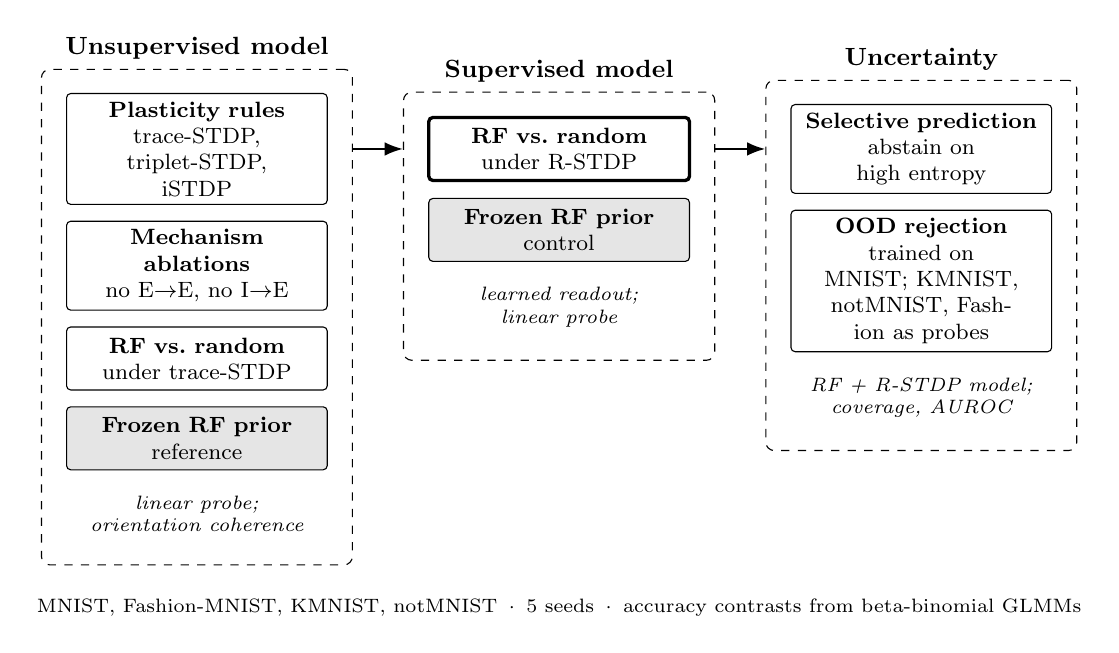
\begin{tikzpicture}[font=\footnotesize, >=Latex,
  item/.style={draw, rounded corners=1.5pt, align=center, text width=31mm,
               inner sep=3pt, minimum height=8mm},
  ref/.style={item, fill=black!10},
  key/.style={item, line width=1.2pt},
  note/.style={font=\scriptsize\itshape, align=center, text width=31mm},
  stage/.style={draw, dashed, rounded corners=3pt, inner sep=3mm},
  arr/.style={->, thick}]

% --- unsupervised model
\node[item] (a1) at (0,0) {\textbf{Plasticity rules}\\trace-STDP, triplet-STDP,\\iSTDP};
\node[item, below=2mm of a1] (a2) {\textbf{Mechanism ablations}\\no E$\to$E, no I$\to$E};
\node[item, below=2mm of a2] (a3) {\textbf{RF vs.\ random}\\under trace-STDP};
\node[ref,  below=2mm of a3] (a0) {\textbf{Frozen RF prior}\\reference};
\node[note, below=2mm of a0] (a4) {linear probe;\\orientation coherence};
\node[stage, fit=(a1)(a4), label={[font=\small\bfseries]above:Unsupervised model}] (P1) {};

% --- supervised model
\node[key] (b0) at (4.6,0) {\textbf{RF vs.\ random}\\under R-STDP};
\node[ref, below=2mm of b0] (b1) {\textbf{Frozen RF prior}\\control};
\node[note, below=2mm of b1] (b2) {learned readout;\\linear probe};
\node[stage, fit=(b0)(b2), label={[font=\small\bfseries]above:Supervised model}] (P2) {};

% --- uncertainty of the trained supervised model
\node[item] (c0) at (9.2,0) {\textbf{Selective prediction}\\abstain on high entropy};
\node[item, below=2mm of c0] (c1) {\textbf{OOD rejection}\\trained on MNIST; KMNIST,\\notMNIST, Fashion as probes};
\node[note, below=2mm of c1] (c2) {RF + R-STDP model;\\coverage, AUROC};
\node[stage, fit=(c0)(c2), label={[font=\small\bfseries]above:Uncertainty}] (P3) {};

\draw[arr] (P1.east |- a1) -- (P2.west |- b0);
\draw[arr] (P2.east |- b0) -- (P3.west |- c0);

\node[anchor=north, font=\scriptsize, yshift=-3mm] at (P2.south |- P1.south)
  {MNIST, Fashion-MNIST, KMNIST, notMNIST \,$\cdot$\, 5 seeds \,$\cdot$\,
   accuracy contrasts from beta-binomial GLMMs};
\end{tikzpicture}
\caption{Experimental design. The unsupervised model is tested against its frozen
receptive-field prior under three plasticity rules and two mechanism ablations, with a
diagnostic RF-versus-random contrast under trace-STDP. The supervised model repeats that
contrast under R-STDP as the confirmatory test, with the frozen prior as a control. The
trained RF + R-STDP model is then evaluated for selective prediction and
out-of-distribution rejection. Grey boxes are frozen references; the bold box is the
confirmatory contrast.}
\label{fig:exp_design}
\end{figure}

\end{document}
